\documentclass[aspectratio=169,xcolor=dvipsnames,10pt]{beamer}
\usetheme{SimpleDarkBlue}
\usepackage[utf8]{inputenc}
\usepackage[english]{babel}
\usepackage{helvet}
\renewcommand{\familydefault}{\sfdefault}
\usepackage{graphicx}
\usepackage{booktabs}
\usepackage{ragged2e}
\usepackage{amsmath,amssymb,amsfonts}
\usepackage{tikz}
\usetikzlibrary{arrows.meta,positioning,fit,calc,shapes.geometric,3d,
                decorations.pathmorphing,decorations.markings}
\usepackage{bm}
\usepackage{listings}
\usepackage{pgfplots}
\pgfplotsset{compat=1.17}
\usepackage{animate}
\usepackage{multimedia}
\usepackage{hyperref}
\usepackage[numbers,sort&compress]{natbib}
\bibliographystyle{unsrtnat}

\setbeamertemplate{frametitle continuation}{}

% Allow more text per slide
\setbeamertemplate{footline}[frame number]

% -----------------------------------------------------------------------------
% METADATA
% -----------------------------------------------------------------------------
\title{FFT-Based Crystal Plasticity\\[4pt]for Polycrystalline Systems}
\subtitle{From Atoms to Algorithms:\\
Physical Model\;\textbullet\;Mathematical Formulation\;\textbullet\;GPU Implementation}
\author{Santiago Garcia Botero}
\institute{University of Texas at San Antonio}
%\titlegraphic{\includegraphics[width=3cm]{utsa_logo.png}}
\date{\today}

% -----------------------------------------------------------------------------
% MACROS
% -----------------------------------------------------------------------------
\newcommand{\bvec}[1]{\mathbf{#1}}
\newcommand{\tens}[1]{\boldsymbol{#1}}
\newcommand{\grad}{\nabla}
\newcommand{\R}{\mathbb{R}}
\newcommand{\taures}{\tau^{\alpha}}
\newcommand{\gammadot}{\dot{\gamma}^{\alpha}}
\newcommand{\dif}{\mathrm{d}}
\newcommand{\avg}[1]{\langle #1 \rangle}
\newcommand{\Ebar}{\bar{\tens{\varepsilon}}}
\newcommand{\Sbar}{\bar{\tens{\sigma}}}
% \newcommand{\xmark}{\textcolor{red}{\ding{55}}}  % requires pifont

\lstset{
  basicstyle=\ttfamily\tiny,
  keywordstyle=\color{NavyBlue}\bfseries,
  commentstyle=\color{OliveGreen},
  stringstyle=\color{BrickRed},
  showstringspaces=false,
  breaklines=true,
  frame=single,
  language=Python,
  numbers=none,
  backgroundcolor=\color{black!5}
}

\begin{document}

% =============================================================================
%  TITLE
% =============================================================================
\begin{frame}
  \titlepage
\end{frame}

% =============================================================================
\begin{frame}{Roadmap}
\justifying

This talk covers three tightly coupled layers:

\vspace{0.6em}
\begin{enumerate}\setlength\itemsep{6pt}
  \item[\textbf{I.}]   \textbf{Physical Model} ---
        What happens inside a metal when you deform it?
        Crystals, dislocations, slip systems, thermal activation, hardening.
  \item[\textbf{II.}]  \textbf{Mathematical Formulation} ---
        How do we turn physics into equations?
        Equilibrium PDE, Lippmann--Schwinger, Green's operator,
        Fourier methods, stress control.
  \item[\textbf{III.}] \textbf{Numerical Implementation} ---
        How do we solve it fast and correctly?
        FFT algorithms, CG acceleration, Anderson mixing,
        discrete derivatives, GPU batching, EVPFFT.
  \item[\textbf{IV.}]  \textbf{Validation \& Results} ---
        Does it work?
        Homogeneous test, polycrystal benchmarks, plasticity fields.
\end{enumerate}

\vspace{0.4em}
\textbf{Goal:} A self-contained GPU-accelerated crystal plasticity simulator
with an interactive GUI.
\end{frame}

% =============================================================================
\begin{frame}{Outline}
  \tableofcontents
\end{frame}

% #############################################################################
%  PART I — PHYSICAL MODEL
% #############################################################################
\section{Physical Model}

% ----------- 1.1 -------------------------------------------------------------
\begin{frame}{Why Crystal Plasticity?}
\justifying

Engineering metals (steel, aluminium, nickel superalloys, titanium) are
\textbf{polycrystalline}: thousands of tiny single crystals (grains)
bonded together, each with a different lattice orientation.

\vspace{0.5em}
\begin{columns}[T]
\begin{column}{0.55\textwidth}
\textbf{The engineering problem:}
\begin{itemize}\setlength\itemsep{2pt}
  \item How does a turbine blade deform under load at $850\,^\circ$C?
  \item Where will fatigue cracks nucleate?
  \item How does sheet metal thin during stamping?
\end{itemize}

\vspace{0.3em}
\textbf{Why not just FEA with J2 plasticity?}
\begin{itemize}\setlength\itemsep{2pt}
  \item J2 knows nothing about grain structure.
  \item Misses anisotropy, texture, hot-spot localisation.
  \item Crystal plasticity resolves \emph{every grain}.
\end{itemize}
\end{column}
\begin{column}{0.42\textwidth}
\centering
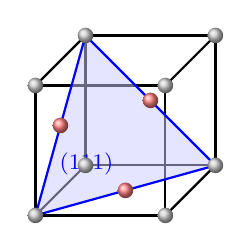
\begin{tikzpicture}[scale=0.55]
  % Unit cell
  \draw[thick] (0,0,0) -- (3,0,0) -- (3,3,0) -- (0,3,0) -- cycle;
  \draw[thick] (0,0,3) -- (3,0,3) -- (3,3,3) -- (0,3,3) -- cycle;
  \draw[thick] (0,0,0)--(0,0,3); \draw[thick] (3,0,0)--(3,0,3);
  \draw[thick] (3,3,0)--(3,3,3); \draw[thick] (0,3,0)--(0,3,3);
  % (111) plane
  \fill[blue!20, opacity=0.5] (3,0,0) -- (0,3,0) -- (0,0,3) -- cycle;
  \draw[blue, thick] (3,0,0) -- (0,3,0) -- (0,0,3) -- cycle;
  \node[blue, font=\footnotesize] at (0.6,0.6,1.5) {$(111)$};
  % Corner atoms
  \foreach \x in {0,3} \foreach \y in {0,3} \foreach \z in {0,3}
    \shade[ball color=gray!40] (\x,\y,\z) circle (0.18);
  % Face centers
  \shade[ball color=red!50] (1.5,1.5,0) circle (0.18);
  \shade[ball color=red!50] (1.5,0,1.5) circle (0.18);
  \shade[ball color=red!50] (0,1.5,1.5) circle (0.18);
\end{tikzpicture}

\vspace{0.2em}
{\footnotesize FCC unit cell with $(111)$ slip plane\\highlighted in blue.}
\end{column}
\end{columns}
\end{frame}

% ----------- 1.2 -------------------------------------------------------------
\begin{frame}{Elastic vs.\ Plastic Deformation}
\justifying

\begin{columns}[T]
\begin{column}{0.55\textwidth}
\textbf{Elastic deformation} (reversible):
\begin{itemize}\setlength\itemsep{2pt}
  \item Stretching of atomic bonds.
  \item Remove load $\to$ shape fully recovers.
  \item Governed by Hooke's law:
        $\tens\sigma = \tens{C}:\tens\varepsilon$.
\end{itemize}

\vspace{0.6em}
\textbf{Plastic deformation} (irreversible):
\begin{itemize}\setlength\itemsep{2pt}
  \item Motion of \textbf{dislocations} ---
        line defects in the crystal lattice.
  \item Remove load $\to$ permanent shape change remains.
  \item Occurs on specific crystallographic planes and directions.
\end{itemize}
\end{column}
\begin{column}{0.42\textwidth}
\centering
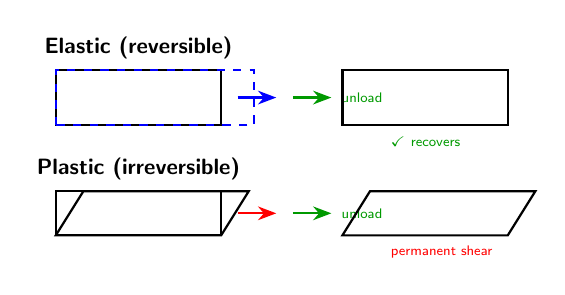
\begin{tikzpicture}[scale=0.7]
  % Elastic
  \node[font=\footnotesize\bfseries] at (1.5,3.4) {Elastic (reversible)};
  \draw[thick] (0,2) rectangle (3,3);
  \draw[thick, blue, -{Stealth}] (3.3,2.5) -- (4.0,2.5);
  \draw[thick, dashed, blue] (0,2) -- (0,3) -- (3.6,3) -- (3.6,2) -- cycle;
  \draw[thick, green!60!black, -{Stealth}] (4.3,2.5) -- (5.0,2.5)
    node[right,font=\tiny] {unload};
  \draw[thick] (5.2,2) rectangle (8.2,3);
  \node[green!60!black,font=\tiny] at (6.7,1.7) {$\checkmark$ recovers};
  % Plastic
  \node[font=\footnotesize\bfseries] at (1.5,1.2) {Plastic (irreversible)};
  \draw[thick] (0,0) rectangle (3,0.8);
  \draw[thick, red, -{Stealth}] (3.3,0.4) -- (4.0,0.4);
  \draw[thick] (0,0) -- (0.5,0.8) -- (3.5,0.8) -- (3.0,0) -- cycle;
  \draw[thick, green!60!black, -{Stealth}] (4.3,0.4) -- (5.0,0.4)
    node[right,font=\tiny] {unload};
  \draw[thick] (5.2,0) -- (5.7,0.8) -- (8.7,0.8) -- (8.2,0) -- cycle;
  \node[red,font=\tiny] at (7.0,-0.3) {permanent shear};
\end{tikzpicture}
\end{column}
\end{columns}
\end{frame}

% ----------- 1.3 -------------------------------------------------------------
\begin{frame}{The FCC Crystal Structure}
\justifying

Most engineering metals (Cu, Al, Ni, Au, $\gamma$-Fe)
have the \textbf{face-centered cubic (FCC)} structure.

\vspace{0.4em}
\begin{columns}[T]
\begin{column}{0.52\textwidth}
\textbf{Key facts:}
\begin{itemize}\setlength\itemsep{3pt}
  \item 4 atoms per unit cell.
  \item Densest-packed planes: $\{111\}$ family (4 planes).
  \item Densest-packed directions: $\langle 110 \rangle$ family.
  \item Dislocations move most easily on dense planes
        in dense directions.
\end{itemize}

\vspace{0.3em}
\textbf{Anisotropy:}\\
Even a single crystal has directional stiffness:
\[
  A = \frac{2C_{44}}{C_{11}-C_{12}}
\]
$A=1$ would be isotropic.
Cu has $A=3.21$ --- very anisotropic!
\end{column}
\begin{column}{0.45\textwidth}
\centering
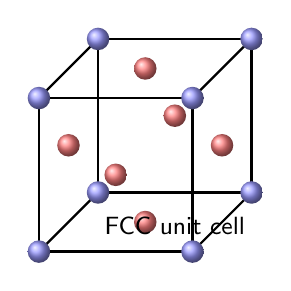
\begin{tikzpicture}[scale=0.65]
  % Cube
  \draw[thick] (0,0,0) -- (3,0,0) -- (3,3,0) -- (0,3,0) -- cycle;
  \draw[thick] (0,0,3) -- (3,0,3) -- (3,3,3) -- (0,3,3) -- cycle;
  \draw[thick] (0,0,0) -- (0,0,3);
  \draw[thick] (3,0,0) -- (3,0,3);
  \draw[thick] (3,3,0) -- (3,3,3);
  \draw[thick] (0,3,0) -- (0,3,3);
  % Corner atoms
  \foreach \x in {0,3} \foreach \y in {0,3} \foreach \z in {0,3}
    \shade[ball color=blue!40] (\x,\y,\z) circle (0.22);
  % Face centers
  \shade[ball color=red!50] (1.5,1.5,0) circle (0.22);
  \shade[ball color=red!50] (1.5,1.5,3) circle (0.22);
  \shade[ball color=red!50] (0,1.5,1.5) circle (0.22);
  \shade[ball color=red!50] (3,1.5,1.5) circle (0.22);
  \shade[ball color=red!50] (1.5,0,1.5) circle (0.22);
  \shade[ball color=red!50] (1.5,3,1.5) circle (0.22);
  \node[below, font=\small] at (1.5,-0.3,0) {FCC unit cell};
\end{tikzpicture}

\vspace{0.4em}
{\small\begin{tabular}{lccc}
\toprule
& $C_{11}$ & $C_{12}$ & $C_{44}$ \\
& (GPa) & (GPa) & (GPa) \\
\midrule
Cu & 168.4 & 121.4 & 75.4 \\
Al & 107.3 & 60.9  & 28.3 \\
Ni & 246.5 & 147.3 & 124.7 \\
\bottomrule
\end{tabular}}
\end{column}
\end{columns}
\end{frame}

% ----------- 1.4 -------------------------------------------------------------
\begin{frame}{Slip Systems: Where Plastic Deformation Happens}
\justifying

A \textbf{slip system} $\alpha$ is a pair: slip plane normal
$\bvec{n}^\alpha$ and slip direction $\bvec{s}^\alpha$.

\vspace{0.3em}
\begin{columns}[T]
\begin{column}{0.50\textwidth}
\textbf{FCC metals have 12 slip systems:}\\
4 planes $\{111\}$ $\times$ 3 directions $\langle 110 \rangle$

\vspace{0.4em}
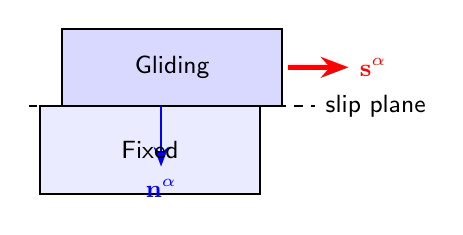
\begin{tikzpicture}[scale=0.70]
    \draw[thick, fill=blue!8] (0,0) rectangle (4,1.6);
    \draw[thick, fill=blue!15] (0.4,1.6) -- (4.4,1.6)
          -- (4.4,3.0) -- (0.4,3.0) -- cycle;
    \draw[-{Stealth[length=3.5mm]}, ultra thick, red]
          (4.5,2.3) -- (5.6,2.3) node[right,font=\small] {$\bvec{s}^\alpha$};
    \draw[dashed, thick] (-0.2,1.6) -- (5.0,1.6)
          node[right,font=\small] {slip plane};
    \draw[-{Stealth[length=2.5mm]}, thick, blue]
          (2.2,1.6) -- (2.2,0.5) node[below=1pt,font=\small] {$\bvec{n}^\alpha$};
    \node[font=\small] at (2,0.8) {Fixed};
    \node[font=\small] at (2.4,2.3) {Gliding};
\end{tikzpicture}

\vspace{0.3em}
The amount of slip on system $\alpha$ is $\gamma^\alpha$.
\end{column}
\begin{column}{0.47\textwidth}
\centering
{\footnotesize\textbf{The 12 FCC slip systems:}}

\vspace{0.2em}
{\tiny\begin{tabular}{clc}
\toprule
$\alpha$ & Plane $\bvec{n}$ & Dir $\bvec{s}$ \\
\midrule
1--3 & $(111)$ & $[01\bar1],[\bar101],[1\bar10]$ \\
4--6 & $(\bar111)$ & $[01\bar1],[101],[\bar1\bar10]$ \\
7--9 & $(1\bar11)$ & $[011],[\bar101],[110]$ \\
10--12 & $(11\bar1)$ & $[011],[101],[\bar110]$ \\
\bottomrule
\end{tabular}}

\vspace{0.3em}
{\footnotesize 4 close-packed $\{111\}$ planes\\$\times$ 3 directions each = 12 systems.}
\end{column}
\end{columns}
\end{frame}

% ----------- 1.5 -------------------------------------------------------------
\begin{frame}{The Schmid Tensor: Projecting Stress onto Slip}
\justifying

Not all stress drives slip equally.  The \textbf{resolved shear stress}
on system $\alpha$ is the projection of the full stress tensor onto the
slip plane:
\[
  \boxed{
    \tau^\alpha = \tens{\sigma} : \tens{P}^\alpha
    = \sigma_{ij}\,P^\alpha_{ij}
  }
\]

where the \textbf{Schmid tensor} is:
\[
  \tens{P}^\alpha
  = \tfrac{1}{2}\bigl(\bvec{s}^\alpha\!\otimes\!\bvec{n}^\alpha
                + \bvec{n}^\alpha\!\otimes\!\bvec{s}^\alpha\bigr)
\]

\vspace{0.3em}
\begin{columns}[T]
\begin{column}{0.52\textwidth}
\begin{itemize}\setlength\itemsep{3pt}
  \item $\tau^\alpha > 0$: forward slip.
  \item $\tau^\alpha < 0$: backward slip.
  \item $|\tau^\alpha|$ small $\to$ system inactive.
\end{itemize}
\end{column}
\begin{column}{0.45\textwidth}
\centering
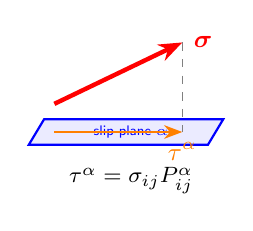
\begin{tikzpicture}[scale=0.65]
  % Stress arrow
  \draw[-{Stealth[length=3mm]}, ultra thick, red] (0,0) -- (2.5,1.2)
    node[right, font=\small] {$\tens\sigma$};
  % Slip plane
  \draw[thick, blue, fill=blue!8] (-0.5,-0.8) -- (3,-0.8)
    -- (3.3,-0.3) -- (-0.2,-0.3) -- cycle;
  \node[blue, font=\tiny] at (1.5,-0.55) {slip plane $\alpha$};
  % Projection
  \draw[dashed, gray] (2.5,1.2) -- (2.5,-0.55);
  \draw[-{Stealth}, thick, orange] (0,-0.55) -- (2.5,-0.55)
    node[below, font=\small] {$\tau^\alpha$};
  % Label
  \node[font=\footnotesize, align=center] at (1.5,-1.5)
    {$\tau^\alpha = \sigma_{ij} P^\alpha_{ij}$};
\end{tikzpicture}

\vspace{0.2em}
{\footnotesize The RSS is the component of stress\\resolved onto the slip direction.}
\end{column}
\end{columns}
\end{frame}

% ----------- 1.6 -------------------------------------------------------------
\begin{frame}{How Much Slip? The Flow Rule}
\justifying

\textbf{Question:} Given $\tau^\alpha$, how fast does dislocation
glide occur?

\vspace{0.4em}
Dislocation motion requires overcoming an \textbf{energy barrier}
$\Delta G$.  At finite temperature $T$, thermal fluctuations help:

\[
  \boxed{
  \dot\gamma^\alpha = \dot\gamma_\text{ref}\;
  \exp\!\Biggl[\!-\frac{\Delta G_0}{k_B T}
  \biggl(1 - \Bigl(\frac{|\tau^\alpha|}{s^\alpha}\Bigr)^{\!p}
  \biggr)^{\!q}\;\Biggr]
  \;\text{sgn}(\tau^\alpha)
  }
\]

\vspace{0.3em}
This is the \textbf{Kocks--Argon--Ashby thermally-activated flow rule},
implemented as the OTIS model in our code.

\vspace{0.3em}
\begin{columns}[T]
\begin{column}{0.48\textwidth}
\textbf{Parameters:}
\begin{itemize}\setlength\itemsep{1pt}\small
  \item $\dot\gamma_\text{ref}=10^{7}\;\text{s}^{-1}$
  \item $\Delta G_0=9.5\times10^{-19}$ J
  \item $p=0.78$, $q=1.15$ (barrier shape)
  \item $s^\alpha$: slip resistance (evolves)
\end{itemize}
\end{column}
\begin{column}{0.48\textwidth}
\centering
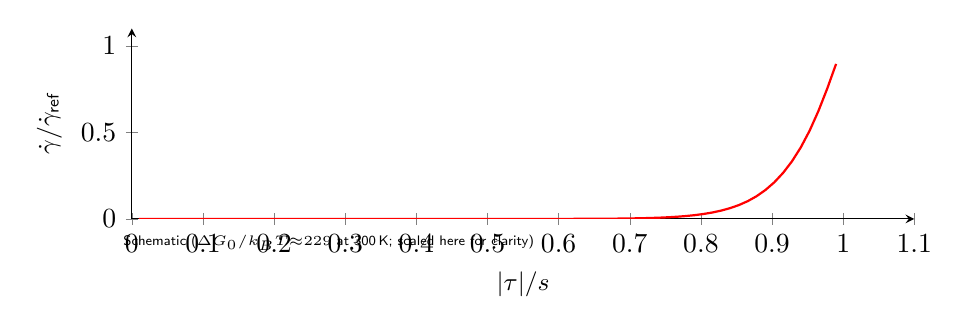
\begin{tikzpicture}
  \begin{axis}[
    width=0.95\textwidth, height=4cm,
    axis lines=left,
    xlabel={\small $|\tau|/s$},
    ylabel={\small $\dot\gamma/\dot\gamma_\text{ref}$},
    domain=0.01:0.99, samples=80,
    xmin=0, xmax=1.1, ymin=0, ymax=1.1,
    ymode=normal,
    no markers,
  ]
    \addplot[thick, red] expression
      {exp(-30*(1-x^0.78)^1.15)};
  \end{axis}
  \node[font=\tiny, align=center] at (2.5,-0.3)
    {Schematic ($\Delta G_0/k_BT{\approx}229$ at 300\,K; scaled here for clarity)};
\end{tikzpicture}
\end{column}
\end{columns}
\end{frame}

% ----------- 1.7 -------------------------------------------------------------
\begin{frame}{Energy Barrier and Temperature Sensitivity}
\justifying

\begin{columns}[T]
\begin{column}{0.48\textwidth}
The barrier shape $(p,q)$ controls \textbf{rate sensitivity}:

\vspace{0.3em}
\centering
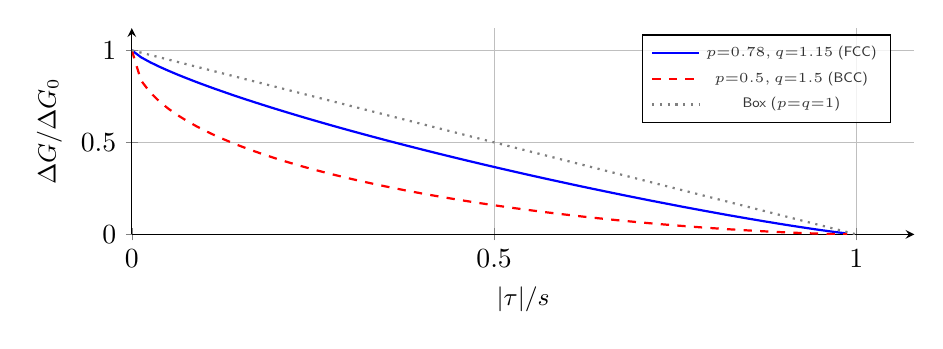
\begin{tikzpicture}
    \begin{axis}[
        width=0.95\textwidth, height=4.2cm,
        axis lines=left,
        xlabel={\small $|\tau|/s$},
        ylabel={\small $\Delta G/\Delta G_0$},
        xtick={0,0.5,1}, ytick={0,0.5,1},
        domain=0:1, samples=80,
        xmin=0, xmax=1.08, ymin=0, ymax=1.12,
        grid=major, no markers,
        legend pos=north east,
        legend style={font=\tiny, fill opacity=0.8},
    ]
        \addplot[thick, blue] expression {(1-x^0.78)^1.15};
        \addlegendentry{$p{=}0.78,q{=}1.15$ (FCC)}
        \addplot[thick, red, dashed] expression {(1-x^0.5)^1.5};
        \addlegendentry{$p{=}0.5,q{=}1.5$ (BCC)}
        \addplot[thick, gray, dotted] expression {(1-x)};
        \addlegendentry{Box ($p{=}q{=}1$)}
    \end{axis}
\end{tikzpicture}
\end{column}
\begin{column}{0.48\textwidth}
\centering
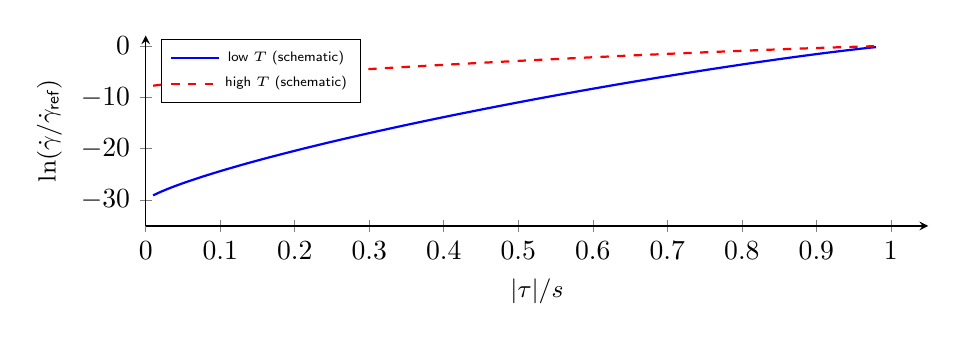
\begin{tikzpicture}
  \begin{axis}[
    width=0.95\textwidth, height=4cm,
    axis lines=left,
    xlabel={\small $|\tau|/s$},
    ylabel={\small $\ln(\dot\gamma/\dot\gamma_\text{ref})$},
    domain=0.01:0.98, samples=100,
    xmin=0, xmax=1.05,
    ymin=-35, ymax=2,
    no markers,
    legend style={font=\tiny, at={(0.02,0.98)}, anchor=north west},
  ]
    \addplot[thick, blue] expression
      {-30*(1-x^0.78)^1.15};
    \addlegendentry{low $T$ (schematic)}
    \addplot[thick, red, dashed] expression
      {-8*(1-x^0.78)^1.15};
    \addlegendentry{high $T$ (schematic)}
  \end{axis}
\end{tikzpicture}

{\footnotesize Higher $T$ $\to$ activation at lower $\tau/s$.\\Coefficients scaled for visual clarity;\\actual $\Delta G_0/k_BT \approx 229$ (300\,K), $\approx 61$ (1123\,K).}
\end{column}
\end{columns}

\vspace{0.3em}
\begin{itemize}\setlength\itemsep{2pt}
  \item At low $\tau/s$: barrier is high $\to$ negligible slip.
  \item Near $\tau \approx s$: barrier vanishes $\to$ rapid slip.
  \item Higher $T$: thermal energy $k_BT$ helps
        overcome the barrier at lower stress.
\end{itemize}
\end{frame}

% ----------- 1.8 -------------------------------------------------------------
\begin{frame}{Plastic Strain from Multiple Slip Systems}
\justifying

The total \textbf{plastic strain rate} is the sum of contributions
from all active systems:
\[
  \boxed{
    \dot{\tens\varepsilon}^p
    = \sum_{\alpha=1}^{12} \dot\gamma^\alpha\,\tens{P}^\alpha
  }
\]

Each system contributes a simple shear along its Schmid tensor.
The superposition produces \textbf{complex, general deformation}.

\vspace{0.3em}
\begin{center}
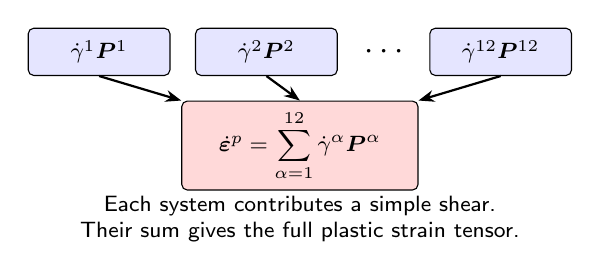
\begin{tikzpicture}[scale=0.85,
  sys/.style={rectangle, draw, rounded corners=2pt, minimum width=1.8cm,
              minimum height=0.6cm, font=\footnotesize, fill=blue!10},
  arr/.style={-{Stealth[length=2mm]}, thick},
]
  \node[sys] (s1) at (0,0) {$\dot\gamma^1 \tens{P}^1$};
  \node[sys] (s2) at (2.5,0) {$\dot\gamma^2 \tens{P}^2$};
  \node[font=\large] at (4.3,0) {$\cdots$};
  \node[sys] (s12) at (6,0) {$\dot\gamma^{12} \tens{P}^{12}$};
  \node[sys, fill=red!15, minimum width=3cm] (sum) at (3,-1.4)
    {$\dot{\tens\varepsilon}^p = \displaystyle\sum_{\alpha=1}^{12} \dot\gamma^\alpha \tens{P}^\alpha$};
  \draw[arr] (s1.south) -- (sum.north west);
  \draw[arr] (s2.south) -- (sum.north);
  \draw[arr] (s12.south) -- (sum.north east);
  \node[font=\footnotesize, align=center] at (3,-2.5)
    {Each system contributes a simple shear.\\Their sum gives the full plastic strain tensor.};
\end{tikzpicture}
\end{center}
\end{frame}

% ----------- 1.9 -------------------------------------------------------------
\begin{frame}{Hardening: Why Metals Get Stronger}
\justifying

As plastic deformation proceeds, \textbf{dislocation density increases}.
Dislocations interact and impede each other $\to$ the crystal \textbf{hardens}.

\vspace{0.3em}
\textbf{Voce hardening law}~\cite{tome1984}:
\[
  \dot{s}^\alpha = \sum_\beta h_{\alpha\beta}\,|\dot\gamma^\beta|,
  \qquad
  h_{\alpha\beta} = q_{\alpha\beta}\;h_0\Bigl(1 - \frac{s^\beta}{s_s}\Bigr)
\]

\begin{columns}[T]
\begin{column}{0.48\textwidth}
\begin{center}\small
\begin{tabular}{llr}
\toprule
\textbf{Parameter} & \textbf{Symbol} & \textbf{Cu value} \\
\midrule
Initial resistance      & $\tau_0$         & 50 MPa  \\
Saturation resistance   & $s_s$            & 200 MPa \\
Initial hardening rate  & $h_0$            & 500 MPa \\
Latent hardening ratio  & $q_\text{lat}$   & 1.4     \\
\bottomrule
\end{tabular}
\end{center}

\vspace{0.2em}
\textbf{Self-hardening} ($\alpha{=}\beta$): $q=1$.\\
\textbf{Latent} ($\alpha{\neq}\beta$): $q=1.4$ (cross-slip interactions).
\end{column}
\begin{column}{0.48\textwidth}
\centering
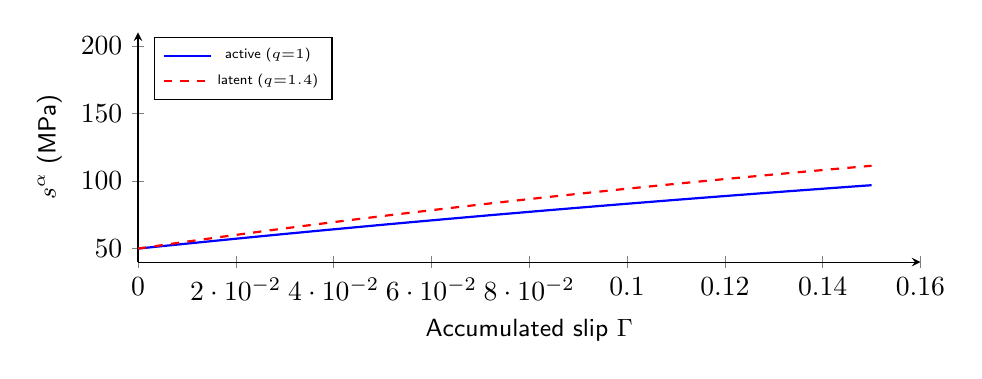
\begin{tikzpicture}
  \begin{axis}[
    width=0.95\textwidth, height=4.5cm,
    axis lines=left,
    xlabel={\small Accumulated slip $\Gamma$},
    ylabel={\small $s^\alpha$ (MPa)},
    domain=0:0.15, samples=60,
    xmin=0, xmax=0.16, ymin=40, ymax=210,
    no markers,
    legend style={font=\tiny, at={(0.02,0.98)}, anchor=north west},
  ]
    \addplot[thick, blue] expression
      {200 - 150*exp(-500/200*x)};
    \addlegendentry{active ($q{=}1$)}
    \addplot[thick, red, dashed] expression
      {200 - 150*exp(-500*1.4/200*x)};
    \addlegendentry{latent ($q{=}1.4$)}
  \end{axis}
\end{tikzpicture}

{\footnotesize Latent hardening is stronger:\\inactive systems harden faster!}
\end{column}
\end{columns}
\end{frame}

% ----------- 1.10 ------------------------------------------------------------
\begin{frame}{Multi-Slip and Emergent Macroscopic Behavior}
\justifying

\begin{columns}[T]
\begin{column}{0.48\textwidth}
\textbf{Multi-slip:}\\
Under general loading, multiple slip systems activate
simultaneously. Their combined effect produces the observed
macroscopic deformation.

\vspace{0.4em}
\centering
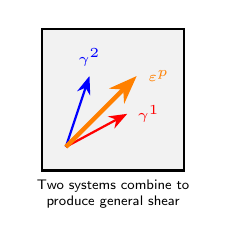
\begin{tikzpicture}[scale=0.6]
  \draw[thick, fill=gray!10] (0,0) rectangle (3,3);
  \draw[-{Stealth}, thick, red] (0.5,0.5) -- (1.8,1.2)
    node[right,font=\tiny] {$\gamma^1$};
  \draw[-{Stealth}, thick, blue] (0.5,0.5) -- (1.0,2.0)
    node[above,font=\tiny] {$\gamma^2$};
  \draw[-{Stealth}, ultra thick, orange] (0.5,0.5) -- (2.0,2.0)
    node[right,font=\tiny] {$\varepsilon^p$};
  \node[font=\tiny, align=center] at (1.5,-0.5)
    {Two systems combine to\\ produce general shear};
\end{tikzpicture}
\end{column}
\begin{column}{0.48\textwidth}
\textbf{Emergent behavior:}\\
Many microscopic slip events (discrete) produce
smooth macroscopic stress-strain curves (continuum).

\vspace{0.4em}
\centering
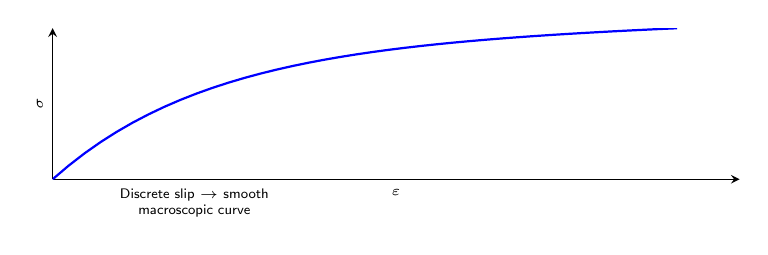
\begin{tikzpicture}
  \begin{axis}[
    width=0.85\textwidth, height=3.5cm,
    axis lines=left,
    xlabel={\tiny $\varepsilon$},
    ylabel={\tiny $\sigma$},
    domain=0:0.1, samples=40,
    xmin=0, xmax=0.11, ymin=0,
    no markers, ticks=none,
  ]
    \addplot[thick, blue] expression
      {200*x + 150*(1-exp(-40*x))};
  \end{axis}
  \node[font=\tiny, align=center] at (1.8,-0.3)
    {Discrete slip $\to$ smooth\\ macroscopic curve};
\end{tikzpicture}
\end{column}
\end{columns}
\end{frame}

% ----------- 1.11 ------------------------------------------------------------
\begin{frame}{Polycrystalline Microstructure}
\justifying

A real metal contains $10^3$--$10^6$ grains.
We represent a \textbf{Representative Volume Element (RVE)} on a regular
$N\times N\times N$ grid.

\vspace{0.3em}
\begin{columns}[T]
\begin{column}{0.52\textwidth}
\textbf{Voronoi tessellation} (periodic):
\begin{enumerate}\setlength\itemsep{2pt}\small
  \item Seed $N_g$ random points in $[0,1)^3$.
  \item Replicate to $3^3$ periodic images.
  \item Assign each voxel to nearest seed (KD-tree).
  \item Random Bunge Euler angles $(\varphi_1,\Phi,\varphi_2)$
        using SO(3) Haar measure.
\end{enumerate}

\vspace{0.2em}
Each grain $g$ has rotation $\bvec{R}_g$ that rotates stiffness
and slip systems into the sample frame:
\[
  C^\text{sample}_{ijkl} = R_{ip}R_{jq}R_{kr}R_{ls}\,C^\text{crystal}_{pqrs}
\]
\end{column}
\begin{column}{0.45\textwidth}
\centering
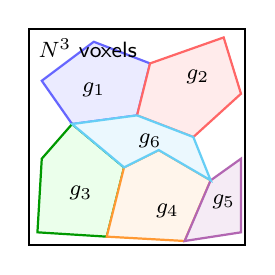
\begin{tikzpicture}[scale=0.55]
  \draw[thick] (0,0) rectangle (5,5);
  \draw[thick,blue!60,fill=blue!8]
    (0.3,3.8)--(1.5,4.7)--(2.8,4.2)--(2.5,3.0)--(1.0,2.8)--cycle;
  \draw[thick,red!60,fill=red!8]
    (2.8,4.2)--(4.5,4.8)--(4.9,3.5)--(3.8,2.5)--(2.5,3.0)--cycle;
  \draw[thick,green!60!black,fill=green!8]
    (0.2,0.3)--(1.8,0.2)--(2.2,1.8)--(1.0,2.8)--(0.3,2.0)--cycle;
  \draw[thick,orange!80,fill=orange!8]
    (1.8,0.2)--(3.6,0.1)--(4.2,1.5)--(3.0,2.2)--(2.2,1.8)--cycle;
  \draw[thick,violet!60,fill=violet!8]
    (3.6,0.1)--(4.9,0.3)--(4.9,2.0)--(4.2,1.5)--cycle;
  \draw[thick,cyan!60,fill=cyan!8]
    (2.5,3.0)--(3.8,2.5)--(4.2,1.5)--(3.0,2.2)%
    --(2.2,1.8)--(1.0,2.8)--cycle;
  \node[font=\footnotesize] at (1.5,3.6) {$g_1$};
  \node[font=\footnotesize] at (3.9,3.9) {$g_2$};
  \node[font=\footnotesize] at (1.2,1.2) {$g_3$};
  \node[font=\footnotesize] at (3.2,0.8) {$g_4$};
  \node[font=\footnotesize] at (4.5,1.0) {$g_5$};
  \node[font=\footnotesize] at (2.8,2.4) {$g_6$};
  \node[font=\footnotesize,anchor=north west] at (0,5) {$N^3$ voxels};
\end{tikzpicture}
\end{column}
\end{columns}
\end{frame}

% ----------- 1.12 ------------------------------------------------------------
\begin{frame}{Local Frames and Slip System Rotation}
\justifying

Each grain has its own crystallographic frame.  To compute the resolved
shear stress, we rotate each slip system into the \textbf{sample frame}:
\[
  \bvec{s}^\alpha_g = \bvec{R}_g\,\bvec{s}^\alpha_\text{crystal},
  \qquad
  \bvec{n}^\alpha_g = \bvec{R}_g\,\bvec{n}^\alpha_\text{crystal}
\]

The Schmid tensor in the sample frame becomes:
\[
  P^\alpha_{g,ij}
  = \tfrac{1}{2}\bigl(s^\alpha_{g,i}\,n^\alpha_{g,j}
  + n^\alpha_{g,i}\,s^\alpha_{g,j}\bigr)
\]

\vspace{0.3em}
\begin{columns}[T]
\begin{column}{0.48\textwidth}
\textbf{This means:}\\
Two grains under the \emph{same} stress tensor will activate
\emph{different} slip systems with \emph{different} magnitudes.

\vspace{0.3em}
$\to$ \textbf{Stress and strain heterogeneity} within the polycrystal.
\end{column}
\begin{column}{0.48\textwidth}
\centering
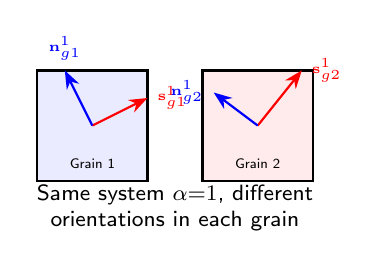
\begin{tikzpicture}[scale=0.7]
  % Grain 1
  \draw[thick, fill=blue!8] (0,0) rectangle (2,2);
  \draw[-{Stealth}, thick, red] (1,1) -- (2.0,1.5)
    node[right,font=\tiny] {$\bvec{s}^1_{g1}$};
  \draw[-{Stealth}, thick, blue] (1,1) -- (0.5,2.0)
    node[above,font=\tiny] {$\bvec{n}^1_{g1}$};
  \node[font=\tiny] at (1,0.3) {Grain 1};
  % Grain 2
  \draw[thick, fill=red!8] (3,0) rectangle (5,2);
  \draw[-{Stealth}, thick, red] (4,1) -- (4.8,2.0)
    node[right,font=\tiny] {$\bvec{s}^1_{g2}$};
  \draw[-{Stealth}, thick, blue] (4,1) -- (3.2,1.6)
    node[left,font=\tiny] {$\bvec{n}^1_{g2}$};
  \node[font=\tiny] at (4,0.3) {Grain 2};
  % Label
  \node[font=\footnotesize, align=center] at (2.5,-0.5)
    {Same system $\alpha{=}1$, different\\orientations in each grain};
\end{tikzpicture}
\end{column}
\end{columns}
\end{frame}

% ----------- 1.13 recap ------------------------------------------------------
\begin{frame}{Part I Summary: The Physical Picture}
\justifying

\begin{center}
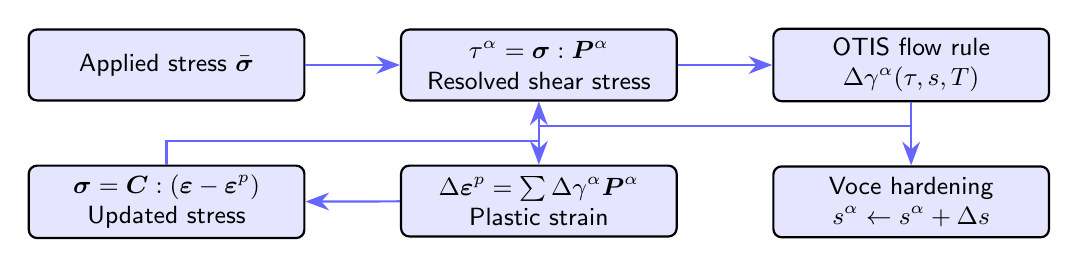
\begin{tikzpicture}[
  box/.style={rectangle, draw, rounded corners=3pt,
              minimum width=3.5cm, minimum height=0.9cm,
              font=\small, align=center, thick, fill=blue!10},
  arr/.style={-{Stealth[length=3mm]}, thick, blue!60},
  node distance=0.5cm
]
  \node[box] (load) {Applied stress $\Sbar$};
  \node[box, right=1.2cm of load] (rss)
    {$\tau^\alpha = \tens\sigma:\tens{P}^\alpha$\\
     Resolved shear stress};
  \node[box, right=1.2cm of rss] (flow)
    {OTIS flow rule\\
     $\Delta\gamma^\alpha(\tau,s,T)$};
  \node[box, below=0.8cm of flow] (hard)
    {Voce hardening\\
     $s^\alpha \leftarrow s^\alpha + \Delta s$};
  \node[box, below=0.8cm of rss] (epsp)
    {$\Delta\tens\varepsilon^p = \sum \Delta\gamma^\alpha \tens{P}^\alpha$\\
     Plastic strain};
  \node[box, below=0.8cm of load] (sig)
    {$\tens\sigma = \tens{C}:(\tens\varepsilon - \tens\varepsilon^p)$\\
     Updated stress};
  \draw[arr] (load) -- (rss);
  \draw[arr] (rss) -- (flow);
  \draw[arr] (flow) -- (hard);
  \draw[arr] (flow.south) -- ++(0,-0.3) -| (epsp.north);
  \draw[arr] (epsp) -- (sig);
  \draw[arr] (sig.north) -- ++(0,0.3) -| (rss.south);
\end{tikzpicture}
\end{center}

\vspace{0.3em}
Every voxel in the RVE runs this loop independently.
The challenge: how to ensure \textbf{equilibrium} and \textbf{compatibility}
across the entire microstructure?
\end{frame}


% #############################################################################
%  PART II — MATHEMATICAL MODEL
% #############################################################################
\section{Mathematical Formulation}

% ----------- 2.1 -------------------------------------------------------------
\begin{frame}{Problem Statement: Equilibrium on an RVE}
\justifying

Given a periodic RVE with spatially varying stiffness $\tens{C}(\bvec{x})$
and prescribed macroscopic stress $\Sbar$,
find the local fields satisfying:

\vspace{0.3em}
\begin{align}
  \text{Equilibrium:}\quad
    & \nabla \cdot \tens{\sigma}(\bvec{x}) = \bvec{0}
    \tag{E1} \\[3pt]
  \text{Constitutive:}\quad
    & \tens{\sigma}(\bvec{x}) = \tens{C}(\bvec{x}) : \tens{\varepsilon}(\bvec{x})
    \tag{E2} \\[3pt]
  \text{Compatibility:}\quad
    & \tens{\varepsilon} = \text{sym}(\nabla \bvec{u}),
      \;\; \bvec{u} \text{ periodic}
    \tag{E3} \\[3pt]
  \text{Average stress:}\quad
    & \avg{\tens{\sigma}} = \Sbar
    \tag{E4}
\end{align}

\vspace{0.3em}
\textbf{Key difficulty:}
$\tens{C}(\bvec{x})$ varies \emph{sharply} between grains ---
each grain has a rotated anisotropic stiffness.

\vspace{0.2em}
\textbf{This is the same PDE that FEM solves} --- we solve it differently
(spectrally), which gives us massive speed advantages on regular grids.
\end{frame}

% ----------- 2.2 -------------------------------------------------------------
\begin{frame}{The Reference Medium Trick}
\justifying

\textbf{Idea:} Decompose $\tens{C}(\bvec{x})$ into a
\emph{known} homogeneous reference $\tens{C}^0$ plus a perturbation:
\[
  \tens{C}(\bvec{x}) = \tens{C}^0 + \Delta\tens{C}(\bvec{x})
\]

The stress can then be split:
\[
  \tens\sigma = \underbrace{\tens{C}^0:\tens\varepsilon}_{\text{reference}}
  + \underbrace{\Delta\tens{C}:\tens\varepsilon}_{\text{polarization }\tens\tau}
\]

\vspace{0.3em}
\textbf{How to choose $\tens{C}^0$?}

\begin{center}\small
\begin{tabular}{lll}
\toprule
\textbf{Mode} & \textbf{Formula} & \textbf{When to use} \\
\midrule
\texttt{mean} (Voigt) & $\tens{C}^0 = \avg{\tens{C}(\bvec{x})}$ & Default, safe \\
\texttt{contrast\_aware} & Geometric mean of per-voxel $K,\mu$ &
  High-contrast composites \\
\bottomrule
\end{tabular}
\end{center}
\end{frame}

% ----------- 2.3 -------------------------------------------------------------
\begin{frame}{Lippmann--Schwinger Equation}
\justifying

Substituting the decomposition into equilibrium and using the
\textbf{Green's function} of the reference medium gives the
\textbf{Lippmann--Schwinger integral equation}~\cite{moulinec1994,moulinec1998}:

\[
  \boxed{
    \tens{\varepsilon}(\bvec{x})
    = \Ebar - \bigl(\tens{\Gamma}^0 * \tens{\tau}\bigr)(\bvec{x})
  }
\]

\vspace{0.3em}
where:
\begin{itemize}\setlength\itemsep{3pt}
  \item $\tens{\Gamma}^0$ is the \textbf{periodic Green's operator}
        of $\tens{C}^0$.
  \item $\tens\tau = \Delta\tens{C}:\tens\varepsilon$ is the
        \textbf{polarization stress}.
  \item $*$ denotes spatial convolution $\to$ \textbf{pointwise
        multiplication in Fourier space}.
\end{itemize}

\vspace{0.3em}
\textbf{This is the key equation.}
Everything that follows is about solving it efficiently.
\end{frame}

% ----------- 2.4 -------------------------------------------------------------
\begin{frame}{The Green's Operator in Fourier Space}
\justifying

For an \textbf{isotropic} reference $(\lambda_0, \mu_0)$,
at wave direction $\bvec{n} = \bvec{\xi}/|\bvec{\xi}|$:

\vspace{0.2em}
\begin{columns}[T]
\begin{column}{0.48\textwidth}
\textbf{Acoustic tensor:}
\[
  A_{ik} = \mu_0\,\delta_{ik} + (\lambda_0{+}\mu_0)\,n_i n_k
\]

\textbf{Analytic inverse:}
\[
  A^{-1}_{ik}
  = \frac{\delta_{ik}}{\mu_0}
  - \frac{\lambda_0{+}\mu_0}{\mu_0(\lambda_0{+}2\mu_0)}\,n_i n_k
\]
\end{column}
\begin{column}{0.48\textwidth}
\textbf{Green's operator} (Fourier space):
\begin{align*}
  b_k &= n_j\,\hat\tau_{kj}
    \\[2pt]
  \hat u_i &= A^{-1}_{ik}\,b_k
    \\[2pt]
  \hat\varepsilon'_{ij}
    &= \tfrac{1}{2}(n_i\hat u_j + n_j\hat u_i)
\end{align*}

Applied pointwise at each frequency $\bvec\xi$.
\end{column}
\end{columns}

\vspace{0.5em}
\textbf{Implementation:} Pre-compute $A^{-1}$ and $\bvec{n}$ at all
$N^3$ frequencies $\to$ stored as $(N,N,N,3,3)$ arrays.
No Voigt notation needed.
\end{frame}

% ----------- 2.5 -------------------------------------------------------------
\begin{frame}{Discrete Derivative Schemes}
\justifying

The wave vector $\hat{k}_i(\xi)$ encodes the spatial derivative
$\partial/\partial x_i$.  Different discretizations are possible:

\vspace{0.3em}
\begin{center}\small
\begin{tabular}{llll}
\toprule
\textbf{Scheme} & \textbf{Wave vector} & \textbf{Reference} & \textbf{Notes} \\
\midrule
\texttt{continuous}
  & $\hat k_i = \xi_i$
  & Classical
  & Exact for smooth fields \\
\texttt{finite\_difference}
  & $\hat k_i = \dfrac{N}{\pi}\sin\!\bigl(\dfrac{\pi\xi_i}{N}\bigr)$
  & Willot 2015~\cite{willot2015}
  & FD-consistent \\
\texttt{rotated}
  & $\hat k_i = N\sin\!\bigl(\dfrac{2\pi\xi_i}{N}\bigr)$
  & Willot \& Pellegrini
  & Best for composites \\
\bottomrule
\end{tabular}
\end{center}

\vspace{0.3em}
\textbf{Why this matters:}
The continuous scheme can produce Gibbs-like ringing at sharp grain
boundaries.  The rotated scheme reduces oscillations and improves
convergence for high-contrast materials.

\vspace{0.2em}
\textbf{In our code:} \texttt{derivative\_scheme='continuous'} is the default;
switch to \texttt{'rotated'} for composites with stiffness contrast $>5\times$.
\end{frame}

% ----------- 2.6 -------------------------------------------------------------
\begin{frame}{Stress-Controlled Loading}
\justifying

FFT solvers are natively \textbf{strain-driven}: input $\Ebar$, output
$\avg{\tens\sigma}$.
To prescribe \textbf{target stress} $\Sbar$, we wrap the solver in a
\textbf{Newton--Raphson iteration} on the macroscopic strain:

\vspace{0.3em}
\begin{enumerate}\setlength\itemsep{4pt}
  \item Initial guess: $\Ebar^{(0)} = (\tens{C}^0)^{-1} : \Sbar$
  \item Solve FFT with $\Ebar^{(k)}$ $\;\to\; \avg{\tens\sigma}^{(k)}$
  \item Residual: $\Delta\Sbar = \Sbar - \avg{\tens\sigma}^{(k)}$
  \item \textbf{Broyden secant update:}
        \[
          \tens{S}_\text{eff}^{(k+1)}
          = \tens{S}_\text{eff}^{(k)}
          + \frac{(\Delta\Ebar - \tens{S}_\text{eff}\Delta\Sbar)
                  \otimes \Delta\Sbar}
                 {\Delta\Sbar \cdot \Delta\Sbar}
        \]
  \item Update: $\Ebar^{(k+1)} = \Ebar^{(k)} + \tens{S}_\text{eff}\,\Delta\Sbar$
\end{enumerate}

\vspace{0.3em}
\textbf{Result:} 4--5 Newton iterations to converge
$\|\Delta\Sbar\|/\|\Sbar\| < 10^{-3}$.
The Broyden update learns the effective compliance as it iterates
--- much better than a fixed Voigt guess.
\end{frame}


% #############################################################################
%  PART III — NUMERICAL IMPLEMENTATION
% #############################################################################
\section{Numerical Implementation}

% ----------- 3.1 -------------------------------------------------------------
\begin{frame}{Basic Scheme (Moulinec--Suquet 1994)}
\justifying

\textbf{Fixed-point iteration} on the Lippmann--Schwinger equation:

\vspace{0.2em}
\begin{enumerate}\setlength\itemsep{2pt}\small
  \item Initialize $\tens{\varepsilon}^{(0)} = \Ebar$
  \item \textbf{Repeat} until
        $\|\Delta\tens\varepsilon\|/\|\tens\varepsilon\| < \text{tol}$:
  \begin{enumerate}\setlength\itemsep{1pt}\small
    \item[a.] $\tens{\sigma}^{(n)} = \tens{C}(\bvec{x}) : \tens{\varepsilon}^{(n)}$
              \hfill (constitutive law)
    \item[b.] $\tens{\tau}^{(n)}
              = \tens{\sigma}^{(n)} - \tens{C}^0 : \tens{\varepsilon}^{(n)}$
              \hfill (polarization)
    \item[c.] $\hat{\tens{\tau}}^{(n)} = \text{FFT}[\tens{\tau}^{(n)}]$
              \hfill (9 forward FFTs)
    \item[d.] $\hat{\tens{\varepsilon}}'
              = \tens{\Gamma}^0(\bvec{\xi}) : \hat{\tens{\tau}}^{(n)}$
              \hfill (pointwise, DC$\,{=}\,0$)
    \item[e.] $\tens{\varepsilon}' = \text{IFFT}[\hat{\tens{\varepsilon}}']$
              \hfill (9 inverse FFTs)
    \item[f.] $\tens{\varepsilon}^{(n+1)} = \Ebar - \tens{\varepsilon}'$
  \end{enumerate}
\end{enumerate}

\vspace{0.3em}
\textbf{Cost per iteration:} $\mathcal{O}(N^3 \log N)$ via FFT
vs.\ $\mathcal{O}(N^6)$ for direct FE assembly.

\vspace{0.2em}
\textbf{Problem:} Converges slowly for high-contrast materials
(many iterations needed).
\end{frame}

% ----------- 3.2 -------------------------------------------------------------
\begin{frame}{CG Acceleration (Zeman 2010)}
\justifying

The basic scheme can be slow.
CG~\cite{zeman2010} reformulates as a linear system
for $\tilde{\tens\varepsilon}$ (strain fluctuation):
\[
  \underbrace{\bigl(\tens{I}
    + \tens{\Gamma}^0 \!\circ\! \Delta\tens{C}\bigr)}_{\tens{A}}\;
  \tilde{\tens\varepsilon}
  = -\tens{\Gamma}^0 \!\circ\! (\Delta\tens{C} : \Ebar)
  \equiv \bvec{b}
\]

\textbf{Conjugate Gradient} solves $\tens{A}\tilde{\tens\varepsilon}=\bvec{b}$
without forming $\tens{A}$ --- only matrix-vector products (2 FFTs each).

\vspace{0.3em}
\begin{columns}[T]
\begin{column}{0.48\textwidth}
\textbf{Advantages over basic scheme:}
\begin{itemize}\setlength\itemsep{2pt}\small
  \item Guaranteed convergence for SPD operators
  \item Superlinear convergence rate
  \item Uses ${\sim}9$ iterations vs.\ ${\sim}14$ basic
\end{itemize}
\end{column}
\begin{column}{0.48\textwidth}
\textbf{Benchmark} (Cu, $16^3$, 8 grains):
\begin{center}\small
\begin{tabular}{lcc}
\toprule
Solver & Iters & Time \\
\midrule
Basic    & 14 & 0.038s \\
CG       &  9 & 0.023s \\
Basic+AA(5) & 10 & 0.046s \\
\bottomrule
\end{tabular}
\end{center}
\end{column}
\end{columns}
\end{frame}

% ----------- 3.3 -------------------------------------------------------------
\begin{frame}{Anderson Acceleration}
\justifying

For the basic scheme, we optionally apply
\textbf{Anderson mixing}~\cite{lucarini2022}
to accelerate convergence:

\vspace{0.3em}
Given the last $m$ iterates $\{x_{k-m+1},\ldots,x_k\}$ and their
fixed-point evaluations $\{G(x_{k-m+1}),\ldots,G(x_k)\}$:

\[
  x_{k+1}
  = G(x_k) - (\Delta\bvec{G})\,\tens\theta^*,
  \qquad
  \tens\theta^*
  = \arg\min_\theta \|F_k - \Delta\bvec{F}\,\theta\|^2
\]

\vspace{0.2em}
where $F_k = G(x_k) - x_k$ is the fixed-point residual,
$\Delta\bvec{F}$ collects the last $m$ residual differences,
and $\Delta\bvec{G} = \Delta\bvec{X} + \Delta\bvec{F}$
(differences of the fixed-point map outputs).

\vspace{0.3em}
\begin{itemize}\setlength\itemsep{3pt}
  \item Window $m=3$--$5$ is typical.
  \item Tikhonov regularization for numerical robustness.
  \item Periodic restart every 50 iterations.
  \item \textbf{Effect:} $\sim$30\% fewer iterations
        (14 $\to$ 10 for polycrystalline Cu).
\end{itemize}
\end{frame}

% ----------- 3.4 -------------------------------------------------------------
\begin{frame}[fragile]{GPU Acceleration: Batched FFT}
\justifying

The FFT solver spends $>60\%$ of runtime in forward/inverse FFTs.
We use \textbf{CuPy} to run all FFTs on the GPU:

\vspace{0.3em}
\begin{columns}[T]
\begin{column}{0.52\textwidth}
\textbf{Batched strategy:}
\begin{enumerate}\setlength\itemsep{2pt}\small
  \item Reshape tensor $(N,N,N,3,3)$
        $\to$ $(9, N,N,N)$.
  \item Run 9 independent 3D FFTs as a batch.
  \item Reshape back to $(N,N,N,3,3)$.
\end{enumerate}

\vspace{0.3em}
\textbf{CPU alternative:} \texttt{use\_rfft=True}
uses real-input FFT (\texttt{rfftn}/\texttt{irfftn}),
which halves memory on the last axis.
\end{column}
\begin{column}{0.45\textwidth}
\begin{lstlisting}[language=Python,basicstyle=\ttfamily\footnotesize]
def fft_3x3(field, use_rfft=False):
    if HAS_GPU:
        N = field.shape[0]
        f9 = field.reshape(N,N,N,9)
        f9 = f9.transpose(3,0,1,2)
        out = cp.empty_like(f9,
                  dtype=cp.complex128)
        for c in range(9):
            out[c] = cpfft.fftn(f9[c])
        return out.transpose(
            1,2,3,0).reshape(
            N,N,N,3,3)
\end{lstlisting}
\end{column}
\end{columns}

\vspace{0.3em}
\textbf{All constitutive operations} (stiffness contraction,
strain updates) also run on GPU via CuPy's NumPy-compatible API.
\end{frame}

% ----------- 3.5 -------------------------------------------------------------
\begin{frame}{EVPFFT: Coupling Plasticity with FFT}
\justifying

The \textbf{elasto-viscoplastic FFT} solver~\cite{lebensohn2001,lebensohn2012}
couples the plastic constitutive update with the FFT equilibrium solver:

\vspace{0.2em}
\begin{enumerate}\setlength\itemsep{2pt}\small
  \item Divide total loading into $N_\text{inc}$ increments.
  \item At each increment:
  \begin{itemize}\setlength\itemsep{1pt}\small
    \item \textbf{Outer Newton loop:} stress control
          ($\Ebar$ updated until $\avg{\tens\sigma} \approx \Sbar$).
    \item \textbf{Inner FFT loop:} fixed-point equilibrium.
    \item At each FFT iteration, every voxel evaluates:
    \begin{itemize}\setlength\itemsep{0pt}\small
      \item $\tau^\alpha = \tens\sigma:\tens{P}^\alpha$
            $\;\to\;$ OTIS flow rule $\;\to\;$ $\Delta\gamma^\alpha$
      \item $\Delta\tens\varepsilon^p
            = \sum_\alpha \Delta\gamma^\alpha\,\tens{P}^\alpha$
      \item $\tens\sigma
            = \tens{C}:(\tens\varepsilon - \tens\varepsilon^p_\text{frozen}
              - \Delta\tens\varepsilon^p)$
    \end{itemize}
    \item After convergence: commit $\tens\varepsilon^p$, update hardening.
  \end{itemize}
\end{enumerate}

\vspace{0.2em}
\textbf{Output:} full-field stress, strain, plastic strain,
slip resistance, and texture evolution at every step.
\end{frame}

% ----------- 3.6 -------------------------------------------------------------
\begin{frame}{EVPFFT: Convergence Acceleration}
\justifying

The EVPFFT loop has two levels that both need fast convergence:

\vspace{0.3em}
\begin{columns}[T]
\begin{column}{0.48\textwidth}
\textbf{Outer (Newton) loop:}
\begin{itemize}\setlength\itemsep{2pt}\small
  \item \textbf{Broyden secant update}:
        learns effective compliance from
        previous Newton steps.
  \item \textbf{Adaptive inner cap}:
        limit FFT iters to 5 early on,
        increase to 15 near convergence.
  \item Result: $\sim$3--5 Newton iters
        per load step.
\end{itemize}
\end{column}
\begin{column}{0.48\textwidth}
\textbf{Inner (FFT) loop:}
\begin{itemize}\setlength\itemsep{2pt}\small
  \item \textbf{Full Newton step}:
        no damping ($\alpha=1$).
  \item \textbf{GPU acceleration}:
        constitutive + FFT on GPU.
  \item 5--15 FFT iters per Newton step.
  \item Total: $\sim$35 constitutive evaluations
        per load step (vs.\ 360 before optimisation).
\end{itemize}
\end{column}
\end{columns}

\vspace{0.3em}
\textbf{10$\times$ speedup} from Broyden + adaptive cap + full step
at 5 GPa loading with OTIS at $T=1123$ K.
\end{frame}

% ----------- 3.7 -------------------------------------------------------------
\begin{frame}{OTIS: The Constitutive Engine}
\justifying

The OTIS flow rule computes $\Delta\gamma^\alpha$ from
$(\tau^\alpha, s^\alpha, T, \Delta t)$:

\vspace{0.2em}
\[
  \Delta\gamma^\alpha
  = \dot\gamma_\text{ref}\;\Delta t\;
  \exp\!\biggl[\!-\frac{\Delta G_0}{k_BT}
  \Bigl(1 - \bigl(|\tau|/s\bigr)^p\Bigr)^q\biggr]
  \;\text{sgn}(\tau^\alpha)
\]

\vspace{0.2em}
\begin{columns}[T]
\begin{column}{0.52\textwidth}
\textbf{Vectorized implementation:}
\begin{itemize}\setlength\itemsep{2pt}\small
  \item Input: $(N_\text{vox}, 12)$ arrays of $\tau$ and $s$.
  \item Saturated regime: $|\tau| \geq s$
        $\to$ $\Delta\gamma = \dot\gamma_\text{ref}\,\Delta t$.
  \item Normal regime: thermally activated exponential.
  \item Clamped to $|\Delta\gamma| \leq 0.005$
        for numerical stability.
  \item Exponent clipped to $\geq -50$
        to avoid underflow.
\end{itemize}
\end{column}
\begin{column}{0.45\textwidth}
\centering
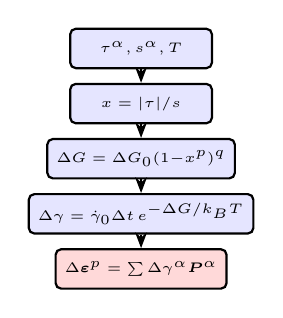
\begin{tikzpicture}[scale=0.7,
  box/.style={rectangle, draw, rounded corners=2pt,
              minimum width=1.8cm, minimum height=0.5cm,
              font=\tiny, align=center, thick, fill=blue!10},
  arr/.style={-{Stealth[length=2mm]}, thick},
]
  \node[box] (tau) at (0,3) {$\tau^\alpha, s^\alpha, T$};
  \node[box] (ratio) at (0,2) {$x = |\tau|/s$};
  \node[box] (bar) at (0,1) {$\Delta G = \Delta G_0(1{-}x^p)^q$};
  \node[box] (exp) at (0,0) {$\Delta\gamma = \dot\gamma_0 \Delta t\, e^{-\Delta G/k_BT}$};
  \node[box, fill=red!15] (out) at (0,-1)
    {$\Delta\tens\varepsilon^p=\sum\Delta\gamma^\alpha \tens{P}^\alpha$};
  \draw[arr] (tau)--(ratio);
  \draw[arr] (ratio)--(bar);
  \draw[arr] (bar)--(exp);
  \draw[arr] (exp)--(out);
\end{tikzpicture}
\end{column}
\end{columns}
\end{frame}

% ----------- 3.8 -------------------------------------------------------------
\begin{frame}{The Analytical OTIS Tangent}
\justifying

For Newton convergence in the constitutive update,
we need $\partial\Delta\gamma/\partial\tau$:

\[
  \frac{\partial\Delta\gamma^\alpha}{\partial\tau^\alpha}
  = \dot\gamma_\text{ref}\,\Delta t\cdot
    \frac{\Delta G_0}{k_BT}\cdot p\cdot q\cdot
    \frac{(|\tau|/s)^{p-1}}{s}\cdot
    \Bigl(1-(|\tau|/s)^p\Bigr)^{q-1}\cdot
    \exp\!\Bigl[\!-\frac{\Delta G_0}{k_BT}
    \bigl(1-(|\tau|/s)^p\bigr)^q\Bigr]
\]

\vspace{0.3em}
\textbf{Why analytical?}
\begin{itemize}\setlength\itemsep{2pt}
  \item Exact --- no truncation error from finite differences.
  \item Fast --- single-pass pointwise evaluation, fully vectorised.
  \item Enables consistent tangent stiffness $\tens{C}^{ep}$ per voxel.
\end{itemize}

\vspace{0.3em}
The tangent is the product of four terms from the chain rule:
\[
  \underbrace{\dot\gamma_\text{ref}\,\Delta t}_{\text{prefactor}}
  \cdot
  \underbrace{\frac{\Delta G_0}{k_BT}}_{\text{thermal}}
  \cdot
  \underbrace{pq\frac{(|\tau|/s)^{p-1}}{s}(1{-}(|\tau|/s)^p)^{q-1}}_{\text{barrier derivatives}}
  \cdot
  \underbrace{\exp[\cdots]}_{\text{exponential}}
\]
\end{frame}

% ----------- 3.9 -------------------------------------------------------------
\begin{frame}{Physics Invariant Checks (Debug Mode)}
\justifying

We implemented automated \textbf{physics sanity checks}
that can be enabled with \texttt{debug\_checks=True}:

\vspace{0.3em}
\begin{center}\small
\begin{tabular}{lll}
\toprule
\textbf{Check} & \textbf{What it verifies} & \textbf{Tolerance} \\
\midrule
\texttt{strain\_symmetry}
  & $\max|\tens\varepsilon - \tens\varepsilon^T| \approx 0$
  & $10^{-10}$ \\
\texttt{stress\_symmetry}
  & $\max|\tens\sigma - \tens\sigma^T| \approx 0$
  & $10^{-10}$ \\
\texttt{macro\_strain\_err}
  & $|\avg{\tens\varepsilon} - \Ebar|/|\Ebar|$
  & $10^{-6}$ \\
\texttt{macro\_stress\_err}
  & $|\avg{\tens\sigma} - \Sbar|/|\Sbar|$
  & $10^{-4}$ \\
\texttt{min\_energy}
  & $\min\bigl(\tfrac{1}{2}\tens\sigma:\tens\varepsilon\bigr) \geq 0$
  & positive \\
\bottomrule
\end{tabular}
\end{center}

\vspace{0.3em}
\textbf{Purpose:} Catch bugs in indexing, Voigt conventions,
or constitutive updates \emph{before} they corrupt the entire simulation.
\end{frame}

% ----------- 3.10 ------------------------------------------------------------
\begin{frame}[fragile]{Per-Iteration Profiler}
\justifying

The \texttt{SolverProfiler} class instruments every phase of the solver
with sub-millisecond timing:

\vspace{0.3em}
\begin{columns}[T]
\begin{column}{0.52\textwidth}
\begin{lstlisting}[language=Python,basicstyle=\ttfamily\footnotesize]
from solver_utils import SolverProfiler

prof = SolverProfiler()

with prof.phase('fft'):
    tau_hat = fft_3x3(tau)

with prof.phase('green_op'):
    gamma_hat = apply_green(tau_hat,
                            n_field, Ainv)

with prof.phase('ifft'):
    gamma = ifft_3x3(gamma_hat)

print(prof.summary("Basic scheme"))
\end{lstlisting}
\end{column}
\begin{column}{0.45\textwidth}
\textbf{Example output:}
\begin{lstlisting}[language={},basicstyle=\ttfamily\footnotesize,keywordstyle={}]
Basic scheme (0.038s total)
  fft           0.014s (36.8%)
  constitutive  0.010s (26.3%)
  ifft          0.008s (21.1%)
  green_op      0.004s (10.5%)
  anderson      0.002s  (5.3%)
\end{lstlisting}

\vspace{0.3em}
\textbf{Use case:}
Identify bottlenecks, validate GPU speedup,
compare solver configurations.
\end{column}
\end{columns}
\end{frame}

% ----------- 3.11 ------------------------------------------------------------
\begin{frame}{Software Architecture}
\justifying

\begin{center}
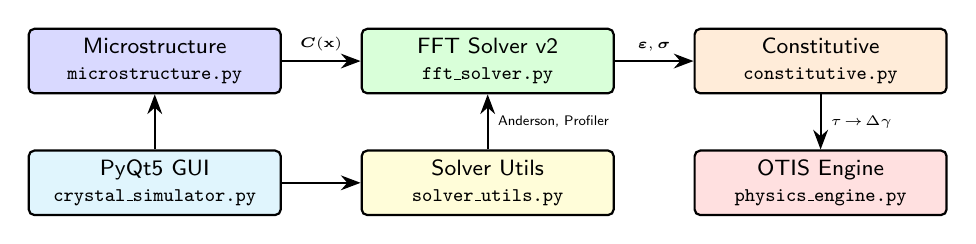
\begin{tikzpicture}[
  box/.style={rectangle, draw, rounded corners=2pt,
              minimum width=3.2cm, minimum height=0.75cm,
              font=\footnotesize, align=center, thick},
  arr/.style={-{Stealth[length=2.5mm]}, thick},
  node distance=0.5cm and 1.0cm
]
  \node[box, fill=blue!15]   (ms)
    {Microstructure\\\texttt{\scriptsize microstructure.py}};
  \node[box, fill=green!15, right=of ms] (fft)
    {FFT Solver v2\\\texttt{\scriptsize fft\_solver.py}};
  \node[box, fill=orange!15, right=of fft] (cp)
    {Constitutive\\\texttt{\scriptsize constitutive.py}};
  \node[box, fill=red!12, below=0.7cm of cp] (otis)
    {OTIS Engine\\\texttt{\scriptsize physics\_engine.py}};
  \node[box, fill=yellow!15, below=0.7cm of fft] (su)
    {Solver Utils\\\texttt{\scriptsize solver\_utils.py}};
  \node[box, fill=cyan!12, below=0.7cm of ms] (gui)
    {PyQt5 GUI\\\texttt{\scriptsize crystal\_simulator.py}};

  \draw[arr] (ms)  -- (fft)
    node[midway,above,font=\tiny] {$\tens{C}(\bvec{x})$};
  \draw[arr] (fft) -- (cp)
    node[midway,above,font=\tiny] {$\tens\varepsilon,\tens\sigma$};
  \draw[arr] (cp)  -- (otis)
    node[midway,right,font=\tiny] {$\tau\!\to\!\Delta\gamma$};
  \draw[arr] (su) -- (fft)
    node[midway,right,font=\tiny] {Anderson, Profiler};
  \draw[arr] (gui) -- (ms);
  \draw[arr] (gui.east) -- (su.west);
\end{tikzpicture}
\end{center}

\vspace{0.3em}
\begin{itemize}\setlength\itemsep{2pt}\small
  \item Pure \textbf{Python 3.11} --- NumPy + CuPy + PyQt5 + PyVista.
  \item \textbf{GPU:} CuPy-CUDA12x on RTX 5070.
  \item Full $(3{\times}3)$ tensor arithmetic
        --- no Voigt-notation pitfalls.
  \item Model-tree GUI with Abaqus-style interaction.
\end{itemize}
\end{frame}

% ----------- 3.12 ------------------------------------------------------------
\begin{frame}{GUI: Interactive Crystal Plasticity Simulator}
\justifying

The \texttt{crystal\_simulator.py} provides a full interactive interface:

\vspace{0.3em}
\begin{columns}[T]
\begin{column}{0.48\textwidth}
\textbf{Model Tree (left panel):}
\begin{itemize}\setlength\itemsep{1pt}\small
  \item \textbf{Material:} $(C_{11}, C_{12}, C_{44})$ + presets
  \item \textbf{Plasticity:} OTIS params ($T$, $\dot\gamma_\text{ref}$,
        $\tau_0$, $s_s$, $h_0$, $q_\text{lat}$)
  \item \textbf{Microstructure:} $N$, grains, seed
  \item \textbf{BCs:} Full stress tensor + presets
  \item \textbf{Solver:} Method, tolerances,
        \texttt{derivative\_scheme},
        \texttt{ref\_medium\_mode},
        Anderson $m$, debug checks
  \item \textbf{Job:} Submit, progress bar
\end{itemize}
\end{column}
\begin{column}{0.48\textwidth}
\textbf{3D Viewer (right panel):}
\begin{itemize}\setlength\itemsep{1pt}\small
  \item PyVista 3D rendering
  \item Field selector:\\
        $\sigma_\text{VM}$, $\sigma_{ij}$,
        $\varepsilon_{ij}$, $|\bvec{u}|$,\\
        $\varepsilon^p_\text{eq}$, accumulated slip,
        slip resistance
  \item Grain boundary overlay
  \item Loading arrows (red/blue)
  \item Step-by-step animation
  \item Dark Fusion theme
\end{itemize}
\end{column}
\end{columns}
\end{frame}


% #############################################################################
%  PART IV — VALIDATION & RESULTS
% #############################################################################
\section{Validation \& Results}

% ----------- 4.1 -------------------------------------------------------------
\begin{frame}{Test 1: Homogeneous Medium --- Exact in 1 Iteration}
\justifying

\textbf{Setup:} Uniform stiffness $\tens{C}=\text{const}$ on $8^3$ grid.
\quad Applied strain: $\varepsilon_{11}=1\%$.

\vspace{0.3em}
\textbf{Expected:} Solver should converge in exactly 1 iteration
with zero error (no heterogeneity $\to$ zero polarization).

\vspace{0.3em}
\begin{center}\small
\begin{tabular}{lccc}
\toprule
\textbf{Derivative scheme} & \textbf{Iterations} &
\textbf{$|\avg\sigma - \sigma_\text{exact}|/|\sigma_\text{exact}|$} &
\textbf{Status} \\
\midrule
\texttt{continuous}        & 1 & $0.00$ & \checkmark \\
\texttt{finite\_difference} & 1 & $0.00$ & \checkmark \\
\texttt{rotated}           & 1 & $0.00$ & \checkmark \\
\bottomrule
\end{tabular}
\end{center}

\vspace{0.4em}
\textbf{Interpretation:}
All three derivative schemes produce the exact analytical solution
for a homogeneous medium.
This verifies the Green's operator, FFT, and stress computation.
\end{frame}

% ----------- 4.2 -------------------------------------------------------------
\begin{frame}{Test 2: Two-Phase Laminate --- Bounds Check}
\justifying

\textbf{Setup:} Layered composite: stiff (Cu) and compliant
($0.5\times$ Cu), equal fractions, $16^3$ grid.

\vspace{0.3em}
\textbf{Expected:} Effective stiffness $C^{\text{eff}}_{11}$
must lie between Reuss (lower) and Voigt (upper) bounds:

\[
  C_\text{Reuss} \leq C_\text{eff} \leq C_\text{Voigt}
\]

\begin{center}\small
\begin{tabular}{lcccl}
\toprule
\textbf{Scheme} & $C_\text{eff}$ (GPa) & Reuss (GPa) & Voigt (GPa)
& \textbf{Status} \\
\midrule
\texttt{continuous} & 112.27 & 112.27 & 126.30 & \checkmark \\
\texttt{rotated}    & 112.27 & 112.27 & 126.30 & \checkmark \\
\bottomrule
\end{tabular}
\end{center}

\vspace{0.3em}
$C_\text{eff}$ sits exactly at the Reuss bound
--- consistent with iso-stress conditions in a laminate
loaded parallel to the layers.
\end{frame}

% ----------- 4.3 -------------------------------------------------------------
\begin{frame}{Test 3: Derivative Scheme Comparison}
\justifying

\textbf{Setup:} Polycrystalline Cu, 8 grains, $16^3$ grid,
$\varepsilon_{11}=1\%$, tol$=10^{-5}$.

\vspace{0.3em}
\begin{center}\small
\begin{tabular}{llcccc}
\toprule
\textbf{Scheme} & \textbf{Solver} & \textbf{Iters} & \textbf{Time (s)}
& \textbf{VM$_\text{max}$ (GPa)} & \textbf{Error} \\
\midrule
continuous        & Basic &  14 & 0.037 & 1.517 & $5.9\times10^{-6}$ \\
continuous        & CG    &   9 & 0.022 & 1.517 & $6.5\times10^{-6}$ \\
finite\_difference & Basic &  14 & 0.038 & 1.521 & $5.8\times10^{-6}$ \\
finite\_difference & CG    &   9 & 0.024 & 1.521 & $6.5\times10^{-6}$ \\
rotated           & Basic &  14 & 0.037 & 1.492 & $6.0\times10^{-6}$ \\
rotated           & CG    &   9 & 0.023 & 1.492 & $6.8\times10^{-6}$ \\
\bottomrule
\end{tabular}
\end{center}

\vspace{0.3em}
\textbf{Observations:}
\begin{itemize}\setlength\itemsep{1pt}\small
  \item CG consistently faster ($9$ vs.\ $14$ iters).
  \item Rotated scheme: slightly lower VM max
        (smoother near grain boundaries).
  \item Same iteration count across schemes ---
        contrast is moderate ($A=3.21$), so all schemes work well.
\end{itemize}
\end{frame}

% ----------- 4.4 -------------------------------------------------------------
\begin{frame}{Test 4: Anderson Acceleration}
\justifying

\textbf{Setup:} Same polycrystal, basic scheme only.
Anderson mixing window $m=0,3,5,8$.

\vspace{0.3em}
\begin{center}\small
\begin{tabular}{cccc}
\toprule
\textbf{Anderson $m$} & \textbf{Iterations} & \textbf{Time (s)}
& \textbf{Final error} \\
\midrule
0 (off)  & 14 & 0.038 & $5.87\times10^{-6}$ \\
3        & 10 & 0.037 & $5.78\times10^{-6}$ \\
5        & 10 & 0.046 & $3.23\times10^{-6}$ \\
8        & 10 & 0.053 & $2.70\times10^{-6}$ \\
\bottomrule
\end{tabular}
\end{center}

\vspace{0.3em}
\textbf{Result:}
\begin{itemize}\setlength\itemsep{2pt}
  \item Anderson reduces iterations by $\sim 30\%$ ($14 \to 10$).
  \item Final error also improves (better accuracy per iteration).
  \item Wall time overhead from the mixing step is small.
  \item Most useful for high-contrast problems where basic scheme
        converges slowly.
\end{itemize}
\end{frame}

% ----------- 4.5 -------------------------------------------------------------
\begin{frame}{Test 5: Stress-Controlled Solver with Broyden}
\justifying

\textbf{Setup:} Polycrystalline Cu, $16^3$,
target $\sigma_{11}=1$ GPa uniaxial.

\vspace{0.3em}
\begin{center}\small
\begin{tabular}{ccccc}
\toprule
\textbf{Newton iter} & $|\Delta\Sbar|/|\Sbar|$ & $\avg{\sigma_{11}}$ (MPa)
& $\avg{\sigma_{22}}$ & $\avg{\sigma_{33}}$ \\
\midrule
0 & $1.3\times10^{-1}$ &  923.0 & 13.3 & 63.7 \\
1 & $3.1\times10^{-2}$ &  978.4 & 19.8 &  1.9 \\
2 & $5.0\times10^{-3}$ &  999.3 &  0.9 & $-$0.2 \\
3 & $1.2\times10^{-3}$ &  999.8 &  0.8 & $-$0.6 \\
4 & $2.1\times10^{-4}$ & 1000.0 &  0.1 &  0.0 \\
\bottomrule
\end{tabular}
\end{center}

\vspace{0.2em}
\textbf{Converged in 5 Newton iterations}, total 45 FFT (CG) iterations,
0.124 seconds.

\vspace{0.2em}
The Broyden secant update quickly learns the effective compliance,
achieving quadratic-like convergence.
Physics checks: all symmetry, macro strain, energy positivity passed.
\end{frame}

% ----------- 4.6 -------------------------------------------------------------
\begin{frame}{Test 6: EVPFFT at High Temperature}
\justifying

\textbf{Setup:} Polycrystalline Cu, $8^3$, 4 grains,
$\sigma_{11} = 5$ GPa, $T = 1123$ K, OTIS flow rule.

\vspace{0.3em}
\begin{columns}[T]
\begin{column}{0.50\textwidth}
\textbf{Solver configuration:}
\begin{itemize}\setlength\itemsep{2pt}\small
  \item 5 load steps (0 $\to$ 5 GPa)
  \item Broyden + adaptive inner cap
  \item $\dot\gamma_\text{ref} = 10^7$ s$^{-1}$
  \item Voce: $\tau_0=50$, $s_s=200$, $h_0=500$ MPa
\end{itemize}

\vspace{0.3em}
\textbf{Results:}
\begin{itemize}\setlength\itemsep{2pt}\small
  \item Total time: $\sim$0.96 s
  \item Max plastic strain: $\sim$10.5\%
  \item $\sim$35 constitutive evaluations per step
\end{itemize}
\end{column}
\begin{column}{0.46\textwidth}
\textbf{What the OTIS flow rule captures:}
\begin{itemize}\setlength\itemsep{2pt}\small
  \item Thermal activation: at $1123$ K,
        dislocations overcome barriers more easily.
  \item Rate sensitivity: $\dot\gamma$ varies
        exponentially with $\tau/s$.
  \item Heterogeneous plastic flow:
        grains oriented for easy slip
        deform more.
\end{itemize}
\end{column}
\end{columns}
\end{frame}

% ----------- 4.7 -------------------------------------------------------------
\begin{frame}{Output Fields: What the Simulator Produces}
\justifying

At every load step, the simulator provides
\textbf{full 3D fields} over the $N^3$ grid:

\vspace{0.3em}
\begin{columns}[T]
\begin{column}{0.48\textwidth}
\textbf{Elastic fields:}
\begin{itemize}\setlength\itemsep{2pt}\small
  \item Von Mises stress $\sigma_\text{VM}$
  \item Stress components $\sigma_{11},\sigma_{22},\ldots$
  \item Strain components $\varepsilon_{11},\varepsilon_{22},\ldots$
  \item Displacement magnitude $|\bvec{u}|$
  \item Hydrostatic pressure
\end{itemize}
\end{column}
\begin{column}{0.48\textwidth}
\textbf{Plastic fields (EVPFFT):}
\begin{itemize}\setlength\itemsep{2pt}\small
  \item Equivalent plastic strain $\varepsilon^p_\text{eq}$
  \item Accumulated slip $\sum|\gamma^\alpha|$
  \item Slip resistance $s^\alpha$ (MPa)
  \item Per-system slip rates $\dot\gamma^\alpha$
\end{itemize}

\vspace{0.2em}
\textbf{All fields} are viewable in the 3D GUI
with step-by-step animation and grain boundary overlay.
\end{column}
\end{columns}
\end{frame}


% #############################################################################
%  PART V — SUMMARY
% #############################################################################
\section{Advanced Physics}

% ----------- 4A.1 ------------------------------------------------------------
\begin{frame}{Finite-Strain Kinematics: $\bvec{F}=\bvec{F}^e\bvec{F}^p$}
\justifying

\textbf{Multiplicative decomposition} replaces infinitesimal strain:
\[
  \bvec{F} = \bvec{F}^e\,\bvec{F}^p,\qquad
  \bvec{E}^e = \tfrac{1}{2}\!\bigl(\bvec{F}^{e\!\top}\bvec{F}^e - \bvec{I}\bigr)
\]

\begin{columns}[T]
\begin{column}{0.48\textwidth}
\textbf{Stress measures:}
\begin{itemize}\setlength\itemsep{2pt}\small
  \item 2nd Piola--Kirchhoff in intermediate config:
        $\bvec{S} = \tens{C}:\bvec{E}^e$
  \item Mandel stress (for resolved shear):
        $\bvec{M} = \bvec{C}^e\bvec{S}$ (non-symmetric)
  \item 1st PK for equilibrium:
        $\bvec{P} = \bvec{F}^e\bvec{S}\bvec{F}^{p{-\!\top}}$
\end{itemize}
\end{column}
\begin{column}{0.48\textwidth}
\textbf{Resolved shear stress:}
\[
  \tau^\alpha = \bvec{M}:(\hat{\bvec{s}}^\alpha\otimes\hat{\bvec{n}}^\alpha)
\]
Slip systems remain \emph{in the crystal frame} ---
$\bvec{F}^e$ carries the lattice rotation implicitly.

\vspace{0.3em}
\textbf{$\bvec{F}^p$ update:}
$\bvec{F}^p_{n+1} =
  (\bvec{I}+\bvec{L}^p\Delta t)\,\bvec{F}^p_n$
with $\bvec{L}^p = \sum_\alpha\!\dot\gamma^\alpha\hat{\bvec{s}}^\alpha\!\otimes\!\hat{\bvec{n}}^\alpha$
\end{column}
\end{columns}
\end{frame}

% ----------- 4A.2 ------------------------------------------------------------
\begin{frame}{Finite-Strain FFT: Unsymmetrised Green Operator}
\justifying

In finite strain, the displacement gradient
$\bvec{H}=\bvec{F}-\bvec{I}=\nabla\bvec{u}$ is \textbf{non-symmetric}
(includes rotation).

\vspace{0.3em}
\textbf{Lippmann--Schwinger:}
$\bvec{H}(\bvec{x}) = \bar{\bvec{H}}
  - \bigl(\bm{\Gamma}^0\ast\bm{\tau}\bigr)(\bvec{x})$,
\quad
$\bm{\tau}=\bvec{P}-\tens{C}^0\!:\!\text{sym}(\bvec{H})$

\vspace{0.5em}
\begin{center}
\begin{tabular}{lcc}
\toprule
& \textbf{Small strain} & \textbf{Finite strain} \\
\midrule
Unknown field & $\varepsilon_{ij}$ (symmetric) & $H_{ij}=F_{ij}-\delta_{ij}$ (non-sym) \\
Stress & $\sigma_{ij}$ (Cauchy) & $P_{ij}$ (1st PK) \\
Green output & $\hat\varepsilon'_{ij}=\tfrac{1}{2}(n_i\hat u_j+n_j\hat u_i)$
             & $\hat H'_{ij}=\hat u_i\,n_j$ \\
Acoustic tensor & $A_{ik}=C^0_{ijkl}n_jn_l$ & identical \\
\bottomrule
\end{tabular}
\end{center}

\vspace{0.3em}
\small Only the \emph{output mapping} changes; the acoustic tensor and its
inverse are \emph{the same} as small strain.
\end{frame}

% ----------- 4A.3 ------------------------------------------------------------
\begin{frame}{Kocks--Mecking Dislocation-Density Hardening}
\justifying

\textbf{Replaces phenomenological Voce} with physically-based dislocation
density evolution (Kocks \& Mecking, 2003):

\vspace{0.3em}
\[
  \dot{\rho}^\alpha
  = \bigl(k_1\sqrt{\textstyle\sum\rho} - k_2\rho^\alpha\bigr)\lvert\dot\gamma^\alpha\rvert
  ,\qquad
  s^\alpha = s_0 + \alpha_T\,\mu\, b\,
  \sqrt{\textstyle\sum_\beta q_{\alpha\beta}\rho^\beta}
\]

\vspace{0.3em}
\begin{columns}[T]
\begin{column}{0.52\textwidth}
\textbf{Cu parameters:}
\begin{itemize}\setlength\itemsep{2pt}\small
  \item $k_1=7\times10^8$ m$^{-1}$ (storage)
  \item $k_2=10$ (dynamic recovery)
  \item $\alpha_T=0.3$ (Taylor coefficient)
  \item $b=2.56\times10^{-10}$ m (Burgers vector)
  \item $\rho_0=10^{12}$ m$^{-2}$ (initial SSD density)
\end{itemize}
\end{column}
\begin{column}{0.44\textwidth}
\textbf{Advantages over Voce:}
\begin{itemize}\setlength\itemsep{2pt}\small
  \item Tracks physical dislocation density
  \item Couples naturally with GND
  \item Temperature dependence via $k_2$
  \item Predicts stage II$\to$III transition
\end{itemize}
\end{column}
\end{columns}
\end{frame}

% ----------- 4A.4 ------------------------------------------------------------
\begin{frame}{Armstrong--Frederick Back-Stress (Bauschinger Effect)}
\justifying

\textbf{Kinematic hardening} introduces a \emph{back-stress} $\chi^\alpha$
on each slip system, capturing the Bauschinger effect:

\vspace{0.3em}
\[
  \dot{\chi}^\alpha = c_1\,\dot\gamma^\alpha
    - c_2\,\chi^\alpha\,\lvert\dot\gamma^\alpha\rvert,
  \qquad\chi_\text{sat}=\frac{c_1}{c_2}
\]

\vspace{0.3em}
\begin{itemize}\setlength\itemsep{3pt}\small
  \item Effective resolved shear stress: $\tau^\alpha_\text{eff}
        = \tau^\alpha - \chi^\alpha$ (fed into OTIS flow rule)
  \item Cu defaults: $c_1=10^9$ Pa, $c_2=10$
        $\Rightarrow\ \chi_\text{sat}=100$ MPa
  \item Armstrong \& Frederick (1966): the simplest nonlinear kinematic
        hardening model that captures load reversal effects
  \item Essential for cyclic loading / fatigue simulations
\end{itemize}
\end{frame}

% ----------- 4A.5 ------------------------------------------------------------
\begin{frame}{Implicit Newton Constitutive Update}
\justifying

\textbf{Per-voxel Newton--Raphson} replaces the explicit constitutive
update---all 12 slip systems are coupled simultaneously:

\vspace{0.3em}
\[
  R^\alpha = \Delta\gamma^\alpha
    - \Delta\gamma^\alpha_\mathrm{OTIS}
      \bigl(\tau^\alpha_\text{eff}(\Delta\bm{\gamma}),\,s,\,T,\,\Delta t\bigr)
    = 0
\]

\textbf{12$\times$12 Jacobian per voxel:}
\[
  J_{\alpha\beta}
  = \delta_{\alpha\beta}
  + \frac{\partial\Delta\gamma^\alpha}{\partial\tau^\alpha}\;
    H_{\alpha\beta},
  \qquad
  H_{\alpha\beta}
    = (\hat{\bvec{s}}^\alpha\otimes\hat{\bvec{n}}^\alpha):
      \tens{C}:
      (\hat{\bvec{s}}^\beta\otimes\hat{\bvec{n}}^\beta)
\]

\begin{itemize}\setlength\itemsep{2pt}\small
  \item $H_{\alpha\beta}$: elastic interaction matrix (constant per grain)
  \item $\partial\Delta\gamma^\alpha/\partial\tau^\alpha$:
        analytical OTIS tangent (slide~7)
  \item Converges in 3--5 Newton iterations (quadratic rate)
  \item Vectorised via \texttt{np.linalg.solve} on $(n_\text{vox},12,12)$
\end{itemize}
\end{frame}

% ----------- 4A.6 ------------------------------------------------------------
\begin{frame}{GND Hardening from Nye Tensor}
\justifying

\textbf{Non-local hardening} from \emph{geometrically necessary dislocations}
(Nye, 1953; Arsenlis \& Parks, 1999):

\vspace{0.3em}
\[
  \bm{\alpha} = \text{curl}(\bvec{F}^p)
  \qquad\Longleftrightarrow\qquad
  \hat{\alpha}_{ij} = \varepsilon_{jkl}\,(i\xi_k)\,\hat{F}^p_{il}
  \quad\text{(spectral)}
\]

\textbf{Projection onto slip systems:}
\[
  \rho^\alpha_\text{edge}
    = \tfrac{1}{b}\,\bm{\alpha}:(\hat{\bvec{s}}^\alpha\otimes\hat{\bvec{t}}^\alpha),
  \qquad
  \rho^\alpha_\text{screw}
    = \tfrac{1}{b}\,\bm{\alpha}:(\hat{\bvec{s}}^\alpha\otimes\hat{\bvec{s}}^\alpha),
  \qquad
  \rho^\alpha_\text{GND}
    = \sqrt{\rho_\text{edge}^2+\rho_\text{screw}^2}
\]

\begin{itemize}\setlength\itemsep{2pt}\small
  \item GND resistance combines with SSD:
        $s = s_0 + \alpha_T\mu b\sqrt{\rho_\text{SSD}+\rho_\text{GND}}$
  \item Computed via FFT-based spectral curl (no finite-difference stencil)
  \item $\hat{\bvec{t}}^\alpha=\hat{\bvec{s}}^\alpha\times\hat{\bvec{n}}^\alpha$
        is the edge dislocation line direction
\end{itemize}
\end{frame}

% ----------- 4A.7 ------------------------------------------------------------
\begin{frame}{Texture Evolution}
\justifying

Crystal orientations \textbf{evolve during deformation} via the elastic
rotation tensor:

\vspace{0.3em}
\[
  \bvec{F}^e = \bvec{R}^e\bvec{U}^e
  \quad\text{(polar decomposition)},
  \qquad
  \bvec{R}_\text{current} = \bvec{R}^e\,\bvec{R}_\text{initial}
\]

\begin{itemize}\setlength\itemsep{3pt}\small
  \item Per-grain averaged $\bvec{F}^e$ gives the lattice rotation
  \item Euler angles updated via $\bvec{R}\to(\varphi_1,\Phi,\varphi_2)$
        (Bunge ZXZ)
  \item Stiffness and slip systems rotate implicitly through $\bvec{F}^e$
        in the Mandel stress formulation
  \item Misorientation field visualised in the GUI
        (degrees from initial orientation)
\end{itemize}

\vspace{0.3em}
\textbf{Validation:} At 1\% uniaxial strain (200~MPa), maximum
misorientation $\approx0.1^\circ$ --- consistent with the elastic regime
(large rotations expected only at $>10\%$ strain).
\end{frame}

\section{Summary \& Future Work}

% ----------- 5.1 -------------------------------------------------------------
\begin{frame}{Summary: What We Built}
\justifying

A \textbf{complete, GPU-accelerated crystal plasticity FFT simulator}
from scratch in Python:

\vspace{0.3em}
\begin{columns}[T]
\begin{column}{0.48\textwidth}
\textbf{Physics:}
\begin{itemize}\setlength\itemsep{2pt}\small
  \item FCC crystal plasticity (12 slip systems)
  \item OTIS thermally-activated flow rule
  \item Voce \emph{and} Kocks--Mecking hardening
  \item Armstrong--Frederick back-stress
  \item Single-crystal elastic anisotropy
  \item \textbf{Finite-strain: $\bvec{F}=\bvec{F}^e\bvec{F}^p$}
  \item \textbf{GND hardening (Nye tensor)}
  \item \textbf{Texture evolution tracking}
\end{itemize}

\vspace{0.3em}
\textbf{Mathematics:}
\begin{itemize}\setlength\itemsep{2pt}\small
  \item Lippmann--Schwinger equation
  \item Green's operator (sym + unsym)
  \item 3 discrete derivative schemes
  \item Broyden stress control
\end{itemize}
\end{column}
\begin{column}{0.48\textwidth}
\textbf{Numerics:}
\begin{itemize}\setlength\itemsep{2pt}\small
  \item Basic + CG solvers
  \item Anderson acceleration
  \item Batched GPU FFT (CuPy)
  \item Implicit Newton (12$\times$12 per voxel)
  \item Per-phase profiling
  \item Physics invariant checks
\end{itemize}

\vspace{0.3em}
\textbf{Software:}
\begin{itemize}\setlength\itemsep{2pt}\small
  \item PyQt5 model-tree GUI
  \item PyVista 3D visualisation
  \item Step-by-step field animation
  \item 21 display fields (stress, strain,
        SSD, GND, back-stress, misorientation)
  \item Pure Python (no Fortran)
\end{itemize}
\end{column}
\end{columns}
\end{frame}

% ----------- 5.2 -------------------------------------------------------------
\begin{frame}{Future Work}
\justifying

\begin{columns}[T]
\begin{column}{0.48\textwidth}
\textbf{Near-term:}
\begin{itemize}\setlength\itemsep{3pt}\small
  \item Exponential map for $\bvec{F}^p$ update
        (preserve $\det\bvec{F}^p=1$)
  \item $64^3$--$128^3$ grids with \texttt{pyFFTW}
  \item HCP crystal structure
        (basal, prismatic, pyramidal slip)
  \item Pole figure output and
        ODF texture analysis
\end{itemize}
\end{column}
\begin{column}{0.48\textwidth}
\textbf{Long-term:}
\begin{itemize}\setlength\itemsep{3pt}\small
  \item Phase-field coupling:
        damage and recrystallisation
  \item Multi-GPU scaling for
        large polycrystals ($256^3$+)
  \item BCC / twin deformation modes
  \item CPFEM--FFT hybrid:
        macro FE with FFT RVE at
        integration points
\end{itemize}
\end{column}
\end{columns}
\end{frame}

% =============================================================================
%  REFERENCES
% =============================================================================
\begin{frame}[allowframebreaks]{References}
  \bibliography{reference}
\end{frame}

% =============================================================================
%  BACKUP / APPENDIX SLIDES
% =============================================================================
\appendix

\begin{frame}{Appendix: Stiffness Rotation Formula}
\justifying

The full 4th-order rotation of the stiffness tensor:
\[
  C^\text{sample}_{ijkl} = R_{ip}R_{jq}R_{kr}R_{ls}\,C^\text{crystal}_{pqrs}
\]

For cubic symmetry, $C^\text{crystal}$ has only 3 independent constants:
$(C_{11}, C_{12}, C_{44})$.  After rotation by Euler angles
$(\varphi_1, \Phi, \varphi_2)$:

\vspace{0.2em}
\begin{itemize}\setlength\itemsep{2pt}\small
  \item The rotation matrix $\bvec{R}$ is $3\times3$ (9 elements).
  \item The contraction involves 81 multiplications per Voigt entry.
  \item We use the Voigt $6\times6$ form:
        $C'_{IJ} = M_{Ii}M_{Jj}\,C_{ij}$
        where $M$ is the $6\times6$ Bond matrix.
\end{itemize}
\end{frame}

\begin{frame}{Appendix: Voigt Notation Conventions}
\justifying

\textbf{Voigt ordering:}
$11 \to 1$, $22 \to 2$, $33 \to 3$,
$23 \to 4$, $13 \to 5$, $12 \to 6$.

\vspace{0.3em}
\textbf{Strain:}
$\varepsilon_\text{Voigt} = (\varepsilon_{11}, \varepsilon_{22},
\varepsilon_{33}, 2\varepsilon_{23}, 2\varepsilon_{13}, 2\varepsilon_{12})$

\vspace{0.3em}
\textbf{Stress:}
$\sigma_\text{Voigt} = (\sigma_{11}, \sigma_{22}, \sigma_{33},
\sigma_{23}, \sigma_{13}, \sigma_{12})$

\vspace{0.3em}
\textbf{Engineering shear factors:}
$\varepsilon_4 = 2\varepsilon_{23}$ (factor of 2 for shear strains).
This ensures $\sigma = C\varepsilon$ works directly with the $6\times6$
stiffness matrix.

\vspace{0.3em}
\textbf{In our code:}
Internal FFT operations use full $(3\times3)$ tensors.
Voigt is used only for storage, I/O, and the constitutive contraction.
Conversion functions: \texttt{strain\_v2t}, \texttt{strain\_t2v},
\texttt{stress\_v2t}, \texttt{stress\_t2v}.
\end{frame}

\end{document}
